\documentclass[parskip=full]{scrartcl}

\pdfoutput=1

\usepackage{breakcites}
\usepackage[square,numbers]{natbib}
\usepackage{float}
\usepackage{graphicx}
\usepackage{geometry}
\geometry{%
	a4paper,
	left=18mm,
	right=18mm,
	top=18mm,
}
\usepackage{amsmath}
\usepackage{enumitem}
\usepackage[ruled,vlined]{algorithm2e}
\usepackage{booktabs}
\usepackage{pgfplotstable}
\pgfplotsset{compat=1.14}
\usepackage{longtable}
\usepackage{tabu}
\usepackage{hyperref}
\date{}

\definecolor{hypecol}{HTML}{0875b7}
\hypersetup{%
    colorlinks,
    linkcolor={hypecol},
    citecolor={hypecol},
    urlcolor={hypecol}
}

\title{%
    Research Trends and Applications of Data Augmentation Algorithms
}

\author{%
	Joao Fonseca\(^{1*}\), Fernando Bacao\(^{1}\)
	\\
	\small{\(^{1}\)NOVA Information Management School, Universidade Nova de Lisboa}
	\\
	\small{*Corresponding Author}
	\\
	\\
	\small{Postal Address: NOVA Information Management School, Campus de
    Campolide, 1070--312 Lisboa, Portugal}
	\\
	\small{Telephone: +351 21 382 8610}
}

\begin{document}

\maketitle

\section{Introduction}

Introduction goes here.

\section{Theory}

Jürgen Schmidhuber's group shows that a simple MLP architecture can achieve
state-of-the-art performance on computer vision benchmarks given strong enough
data augmentation [1,2].

[1] Better digit recognition with a committee of simple Neural Nets. Meier,
Cires, Gambardella and Schmidhuber 2011 [PDF]

[2] Handwritten Digit Recognition with a Committee of DeepNeural Nets on GPUs.
Ciresan, Meier, Gambardella and Schmidhuber 2011 [PDF]

\section{Methodology}

In this section we describe the procedures defined for the literature
collection, data preprocessing and literature analysis. The analysis of the
literature was developed with 3 different approaches. Throughout the
analyses, data preprocessing and hyperparameter tuning was developed
iteratively. The procedure adopted in this manuscript is shown in
Figure~\ref{fig:slr_diagram}.

The literature collection procedure is described in
Subsection~\ref{sec:lit_collection}. The data and text preprocessing is
described in Subsection~\ref{sec:data_preprocessing}. The exploratory data
analysis described in Subsection~\ref{sec:journal_and_conference_analysis} was
done to understand which manuscripts, journals and conferences are most
significant within the field of Data Augmentation. The manuscripts' keywords
were used to construct a network of keywords (described in
Subsection~\ref{sec:keyword_analysis}) and study the different communities of
keywords found in the network. The topic modelling and parameter tunning is described in
Subsection~\ref{sec:topic_modelling}. The abstract embeddings procedure is
described in Subsection~\ref{sec:abstract_embeddings}.

\begin{figure}[H]
	\centering
	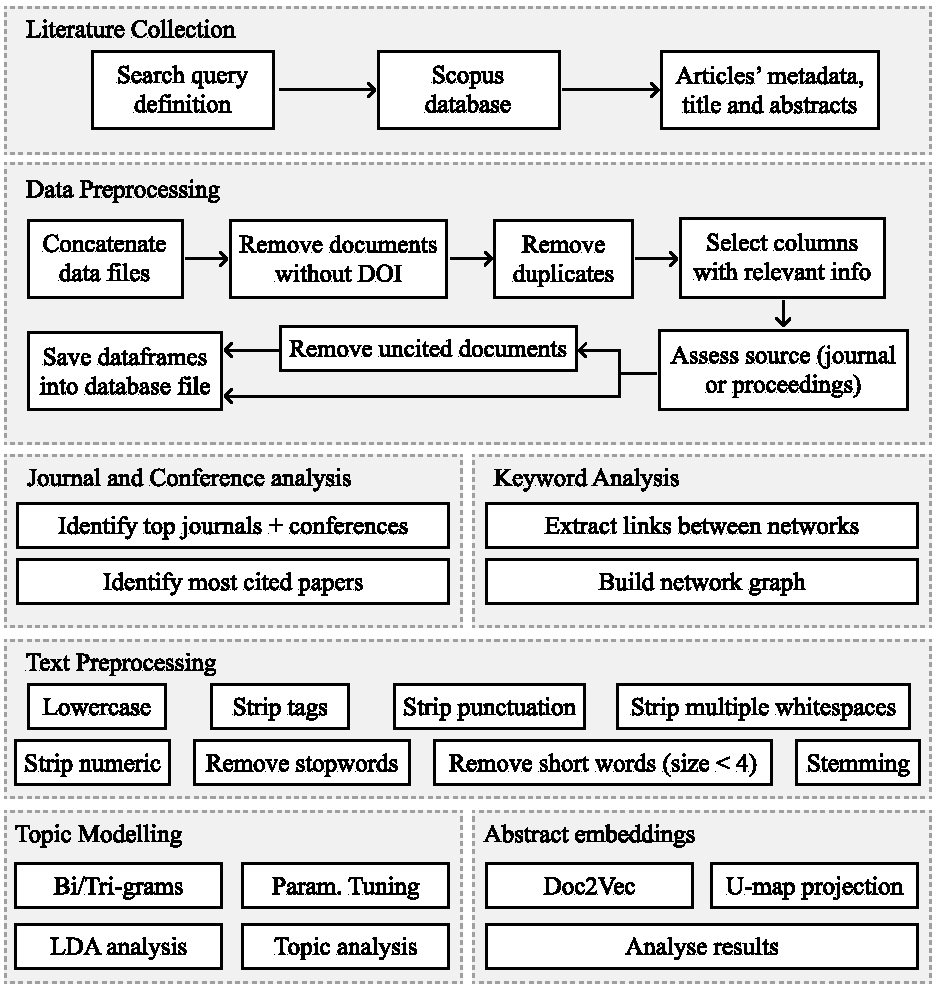
\includegraphics[width=.75\linewidth]{../analysis/slr_diagram}
    \caption{Diagram of the proposed literature analysis approach.
    }~\label{fig:slr_diagram}
\end{figure}

\subsection{Literature Collection}~\label{sec:lit_collection}

The focus of this literature analysis is to understand the different
algorithms, domains and/or tasks that employ data augmentation techniques.
Therefore, we use the keyword ``data augmentation'' in order to ensure an
unbiased analysis. The results were then limited to conference papers and
journal articles written in English that were published in the past 15 years.
Due to the large amount of results found, using using solely the
\href{https://www.scopus.com/}{Scopus} database was found to be sufficient.
The resulting query is shown below:

\begin{verbatim}
    KEY ( "data augmentation" )  AND  ( LIMIT-TO ( LANGUAGE ,  "English" ) )  
    AND ( LIMIT-TO ( DOCTYPE ,  "cp" )  OR  LIMIT-TO ( DOCTYPE ,  "ar" ) )  
    AND  (
            LIMIT-TO ( PUBYEAR ,  2021 )  OR  LIMIT-TO ( PUBYEAR ,  2020 )  
        OR  LIMIT-TO ( PUBYEAR ,  2019 )  OR  LIMIT-TO ( PUBYEAR ,  2018 )  
        OR  LIMIT-TO ( PUBYEAR ,  2017 )  OR  LIMIT-TO ( PUBYEAR ,  2016 )  
        OR  LIMIT-TO ( PUBYEAR ,  2015 )  OR  LIMIT-TO ( PUBYEAR ,  2014 )  
        OR  LIMIT-TO ( PUBYEAR ,  2013 )  OR  LIMIT-TO ( PUBYEAR ,  2012 )  
        OR  LIMIT-TO ( PUBYEAR ,  2011 )  OR  LIMIT-TO ( PUBYEAR ,  2010 )  
        OR  LIMIT-TO ( PUBYEAR ,  2009 )  OR  LIMIT-TO ( PUBYEAR ,  2008 )  
        OR  LIMIT-TO ( PUBYEAR ,  2007 )  OR  LIMIT-TO ( PUBYEAR ,  2006 ) 
    )  
\end{verbatim}

The resulting data selection/filtering pipeline is shown in
Figure~\ref{fig:data_filtering_pipeline}. Due to the limitations in the Scopus
data export (maximum 2000 documents per export), the data was split in four
different time periods and exported separately: 2006 until 2018, 2019, 2020
and 2021, which produced four CSV files.

\subsection{Data Preprocessing}~\label{sec:data_preprocessing}

The data preprocessing stage and amount of documents dropped is represented in
Figure~\ref{fig:data_filtering_pipeline}. The data was first concatenated into
a single data frame. During this process, we found that one of the exported
references had a corrupted line, which caused the loss of one additional
document.  Since the DOI can be used as a unique identifier for intellectual
property~\cite{Paskin1999}, references without a DOI were disregarded from
further analysis, while the ones with the same identifiers are removed
(\textit{i.e.}, only one of the repeating entries is kept).

This dataset was kept to perform the analysis described in
Subsection~\ref{sec:journal_and_conference_analysis}. However, further
preprocessing was done for the remaining parts of the literature analysis.
References without any citations were excluded for the keyword network and
topic modelling analyses. Finally, only the documents containing keywords in
Scopus' database were used to prepare the network analysis.

\begin{figure}[H]
	\centering
    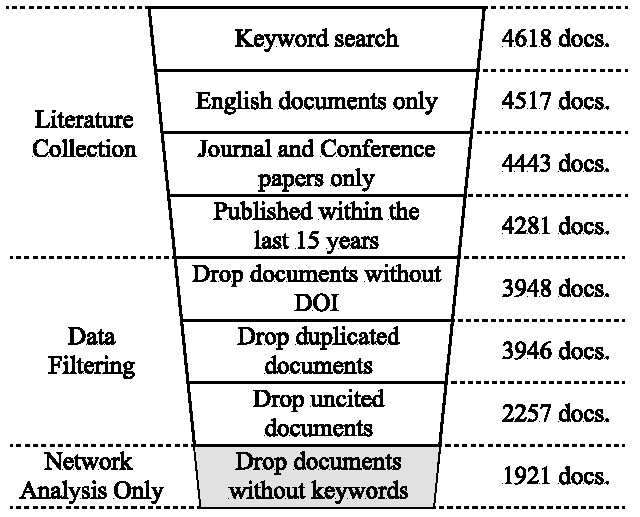
\includegraphics[width=.55\linewidth]{../analysis/data_filtering_pipeline}
    \caption{Data filtering pipeline.
    }~\label{fig:data_filtering_pipeline}
\end{figure}

\subsection{Journal and Conference analysis}~\label{sec:journal_and_conference_analysis}

The exploratory analysis developed on the preprocessed dataset was targeted
towards the identification of the most significant works, journals and
conferences. We used the citation count as a proxy to understand the impact of
a specific manuscript within the research community.

The identification of the most significant conferences and journals is done by
sorting each type of publication according to the number of citations per
document. Conferences and journals with less than 10 papers published in the
area are not considered in this analysis. 

\subsection{Keyword Analysis}~\label{sec:keyword_analysis}

The analysis of keywords is expected to uncover general trends in data
augmentation research and its applications. The keyword ``data augmentation''
was removed since it would link with all other keywords. Keywords are
connected based on their co-occurrence in each research paper to form the
edges of the network.  It consists of an undirected graph whose weights are
based on the total citation count for the papers containing a given keyword
pair and is calculated as $\textrm{weight} = \log(\textrm{citations}) + 1$ to
avoid a potential bias caused by highly cited research articles.

Keyword combinations showing up in only one document are removed from further
analysis. The keyword network is then analysed using Python and the
communities were found using the greedy modularity maximization algorithm
proposed in~\cite{Clauset2004}. The results of the analysis and community
detection were ported to Gephi to produce the final visualizations.

\subsection{Topic Modelling}~\label{sec:topic_modelling}

The extraction of topics was done using the publication's abstracts. The words
were tokenized and all tags, special characters, punctuation, multiple white
spaces, numeric values, stop words and words with size smaller than 4 were
removed. Finally, we enriched the corpus by constructing bi-grams and
tri-grams.

We used a Latent Dirichlet Allocation (LDA) model~\cite{Pritchard2000} to
infer the topics present in our research domain. The tuning of the parameters
was done through experimentation and qualitative interpretation of the results
achieved. Additionally, the area under the coherence score curve shown in
Figure~\ref{fig:lda_coherence_analysis} was also used as a reference for
parameter tuning and the choice of parameters is described in
Table~\ref{tab:hyperparameters}. 

\begin{figure}[H]
	\centering
    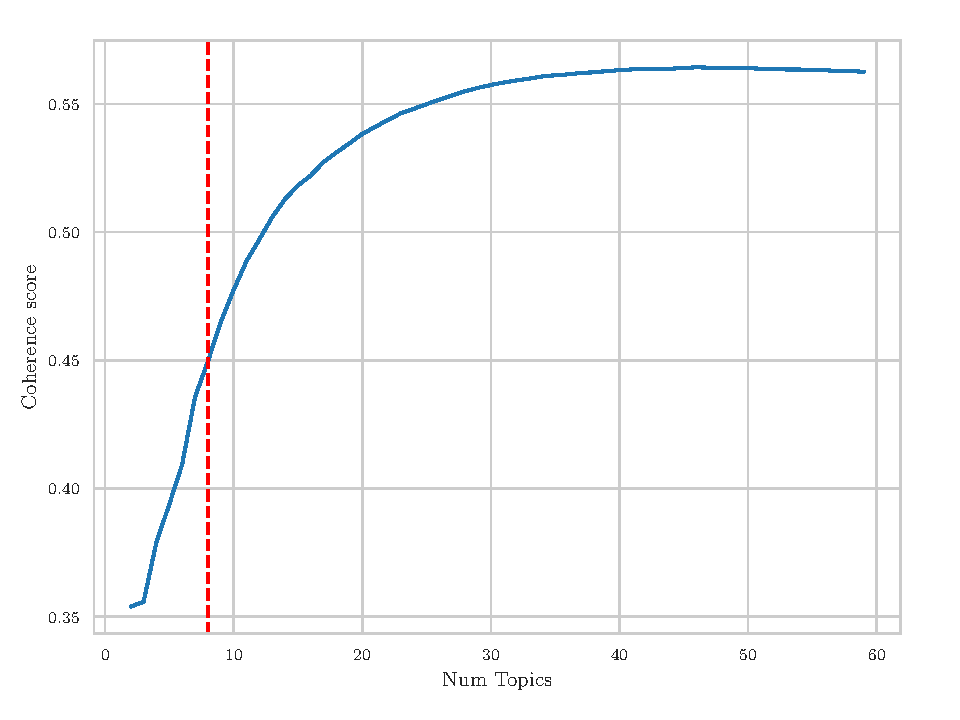
\includegraphics[width=.9\linewidth]{../analysis/lda_coherence_analysis}
    \caption{%
        Analysis of the average coherence scores on an optimized LDA model
        with varying number of topics. The red dotted line represents the
        number of topics chosen for the final model. The coherence score curve
        using the average coherence of 5 different initializations over each
        number of topics.
    }~\label{fig:lda_coherence_analysis}
\end{figure}

\subsection{Abstract embeddings}~\label{sec:abstract_embeddings}

The embeddings of the abstracts was done using the Doc2Vec
algorithm~\cite{Le2014} and the hyperparameters are defined in
Table~\ref{tab:hyperparameters}. This allowed the representation of the corpus
in a 25 dimension space and was further reduced using a
U-map~\cite{Mcinnes2018} to allow the visualization of the output in a
2-dimensional space.

\begin{table}[H]
    \centering
    \begin{tabular}{lll}
        \toprule
        Model   &   Hyperparameter  &   Value \\
        \midrule
        LDA     &   Num Topics      &   8     \\
                &   Chunk Size      &   2000  \\
                &   Passes          &   20    \\
                &   Alpha           &   0.1   \\
                &   ETA             &   auto  \\
        \midrule
        Doc2Vec &   Size            &   25    \\
                &   Iterations      &   100   \\
                &   Min count       &   10    \\
        \bottomrule
    \end{tabular}
    \caption{Hyperparameters used.}~\label{tab:hyperparameters}
\end{table}

\subsection{Software Implementation}~\label{sec:software_implementation}

The analysis and modelling was developed using the Python programming
language, along with the
\href{https://scikit-learn.org/stable/}{Scikit-Learn}~\cite{Pedregosa2011},
\href{https://radimrehurek.com/gensim/}{Gensim}~\cite{Rehurek2010},
\href{https://github.com/lmcinnes/umap}{Umap-Learn}~\cite{Mcinnes2018} and
\href{https://networkx.org/}{Networkx}~\cite{Hagberg2008} libraries. The final
network analysis and visualization was done with
\href{https://gephi.org/}{Gephi}~\cite{Bastian2009}. All functions,
algorithms, analyses and results are provided in the
\href{https://github.com/joaopfonseca/research}{GitHub repository of the
project}.

\section{Results}

The popularity of research in data generation has grown significantly in the
past 5 years, as shown in Figure~\ref{fig:area_chart_cited_documents}. Despite
the significant amount of uncited publications, out of the ones published in
2021 up to this date,\textbf{\ XX\%} have already been used in other works.

\begin{figure}[H]
	\centering
    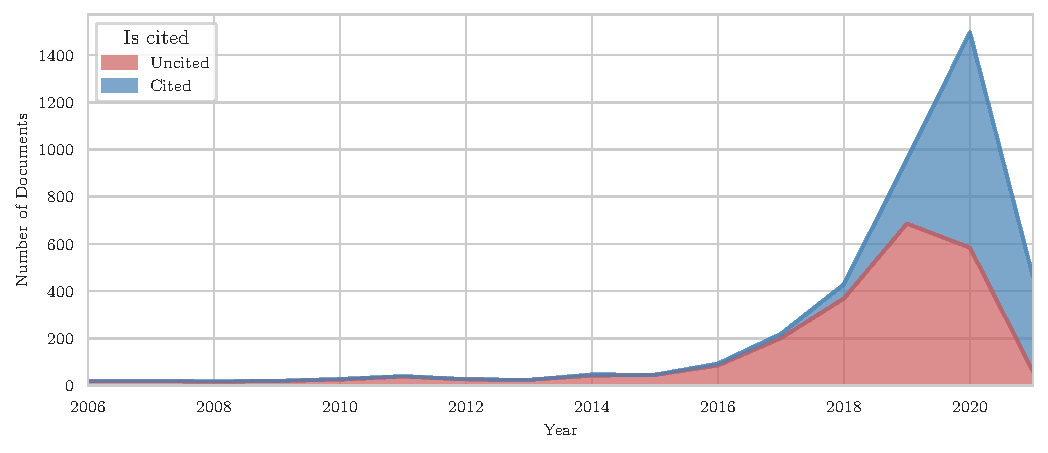
\includegraphics[width=\linewidth]{../analysis/area_chart_cited_documents}
    \caption{Annual number of publications containing the keyword ``data
        generation''.
    }~\label{fig:area_chart_cited_documents}
\end{figure}

%\subsection{Terms Frequency}

\subsection{Journal and Conference Analysis}

\begin{table}
    \centering
    \pgfplotstabletypeset[
    	begin table=\begin{longtable},
    	end table=\end{longtable},
        col sep=semicolon,
        string type,
        every head row/.style={%
            before row=\toprule,
            after row=\midrule
        },
        every last row/.style={after row=\bottomrule},
        string type,
    ]{../analysis/top_journals.csv}
    \vspace{.2cm}
    \caption{\label{tab:top_journals}
        Top journals focusing on data augmentation techniques.
    }
\end{table}

\begin{table}
    \centering
    \pgfplotstabletypeset[
    	begin table=\begin{longtable},
    	end table=\end{longtable},
        col sep=semicolon,
        string type,
        every head row/.style={%
            before row=\toprule,
            after row=\midrule
        },
        every last row/.style={after row=\bottomrule},
        string type,
        columns/Source title/.style={column type={p{.4\linewidth}}},
    ]{../analysis/top_conferences.csv}
    \vspace{.2cm}
    \caption{\label{tab:top_conferences}
        Top conferences focusing on data augmentation techniques.
    }
\end{table}

\subsection{Most Cited Publications}

\begin{table}
    \centering
    \pgfplotstabletypeset[
    	begin table=\begin{longtable},
    	end table=\end{longtable},
        col sep=semicolon,
        string type,
        every head row/.style={%
            before row=\toprule,
            after row=\midrule
        },
        every last row/.style={after row=\bottomrule},
        string type,
        columns/Authors/.style={column type={p{.25\linewidth}}},
        columns/Title/.style={column type={p{.4\linewidth}}},
        columns/Year/.style={column type={p{.05\linewidth}}},
        columns/Cited by/.style={column type={p{.09\linewidth}}}
    ]{../analysis/top_papers.csv}
    \vspace{.2cm}
    \caption{\label{tab:top_papers}
        Top papers using data augmentation techniques.
    }
\end{table}


\subsection{Keyword Analysis}

This can be done by text occurrence network visualization or embeddings.

\begin{figure}[H]
	\centering
    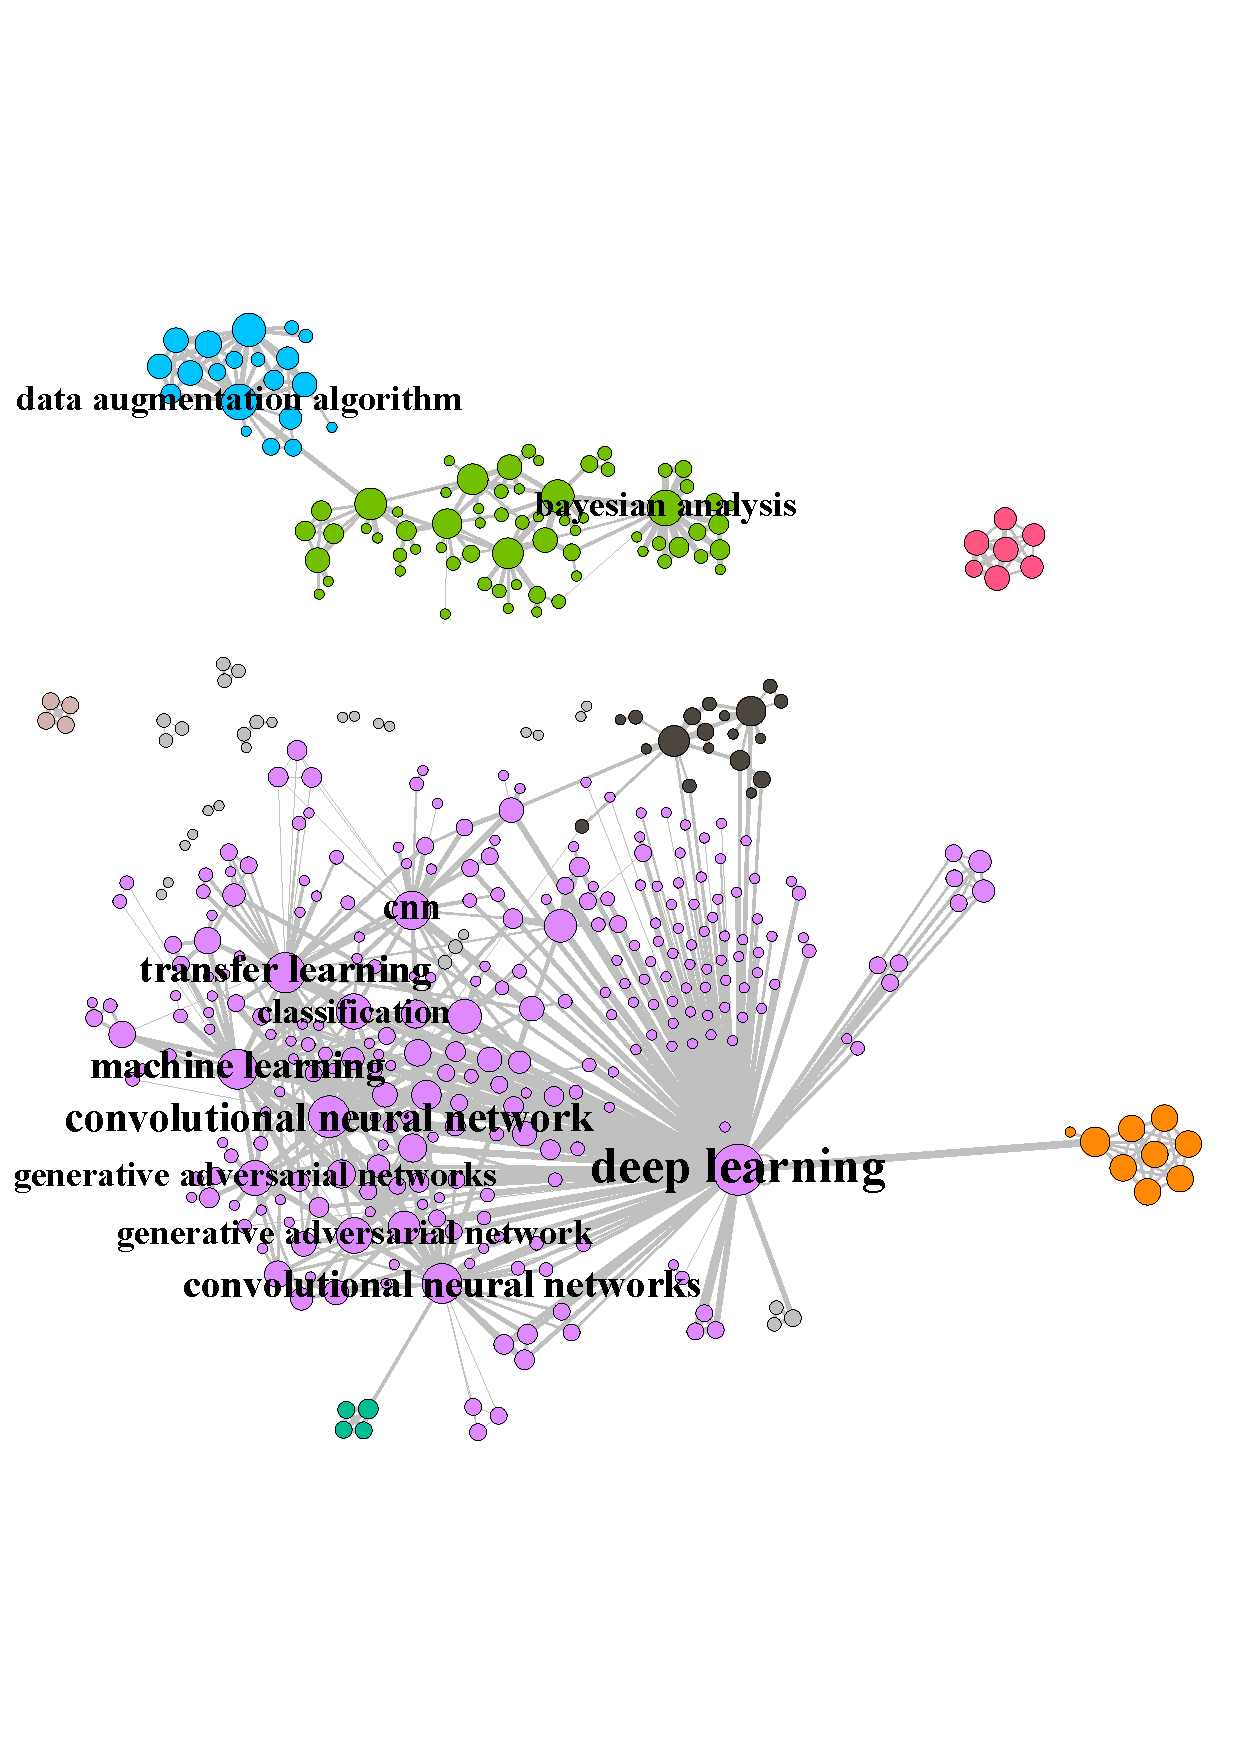
\includegraphics[width=\linewidth]{../analysis/keyword_network}
    \caption{Keyword network.
    }~\label{fig:keyword_network}
\end{figure}



\subsection{Topic Analysis}

LDA analysis goes here

\begin{figure}[H]
	\centering
    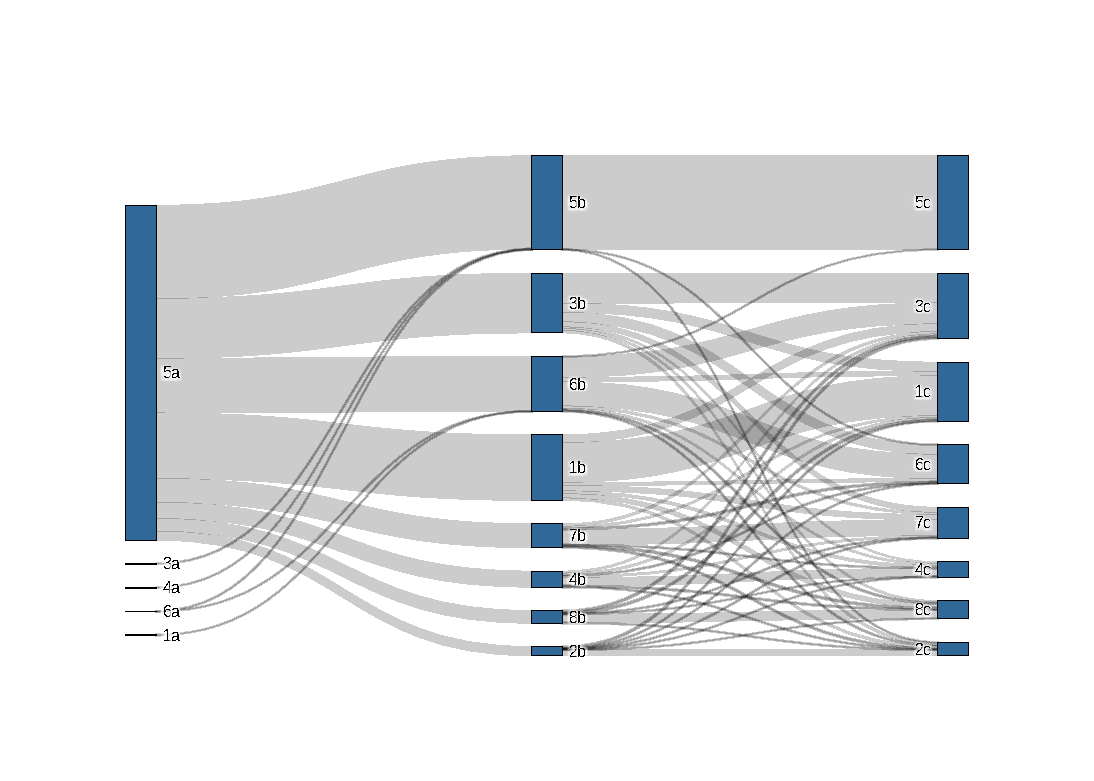
\includegraphics[width=\linewidth]{../analysis/lda_topics_sankey}
    \caption{Distribution of documents over the different topics found. The
        left column represent the primary topics, the middle column represents
        the secondary topics and the right columns represents the tertiary
        topics.
    }~\label{fig:lda_topics_sankey}
\end{figure}

\begin{table}
    \centering
    \pgfplotstabletypeset[
    	begin table=\begin{longtable},
    	end table=\end{longtable},
        col sep=semicolon,
        string type,
        every head row/.style={%
            before row=\toprule,
            after row=\midrule
        },
        every last row/.style={after row=\bottomrule},
        string type,
        columns/Representative Paper/.style={column type={p{.4\linewidth}}},
        columns/Words/.style={column type={p{.35\linewidth}}},
    ]{../analysis/topic_analysis.csv}
    \vspace{.2cm}
    \caption{\label{tab:topic_analysis}
        Description of the main topics found in the literature.
    }
\end{table}

\begin{figure}[H]
	\centering
    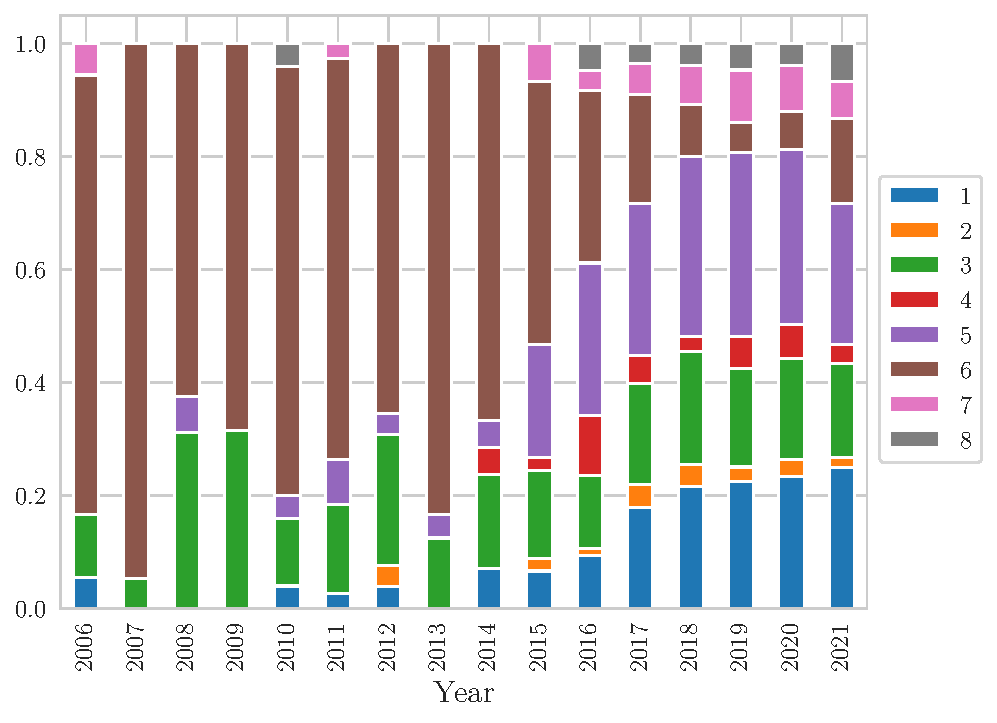
\includegraphics[width=\linewidth]{../analysis/topics_per_year}
    \caption{Topic frequency per year.
    }~\label{fig:topics_per_year}
\end{figure}

\subsection{Abstract embeddings}

\begin{figure}[H]
	\centering
    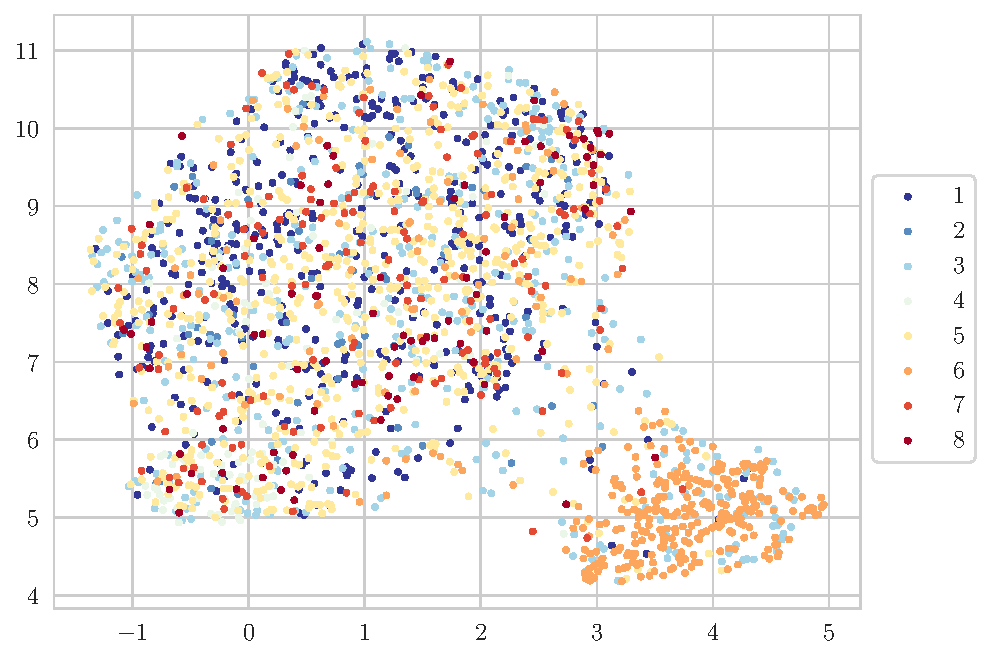
\includegraphics[width=\linewidth]{../analysis/umap_lda_topics}
    \caption{Document embeddings discriminated by LDA topic.
    }~\label{fig:umap_lda_topics}
\end{figure}

\subsection{Application and Method Analysis}

\section{Discussion}

Discussion goes here.

\subsection{Research Question Discussion}

\subsection{Research Gap Discussion}

\subsection{Study Limitation Discussion}

\section{Conclusions}

\bibliography{references}
% \bibliographystyle{apalike}
\bibliographystyle{ieeetr}

\end{document}
